\section{Week 3 - Sequence models \& Attention mechanism}
\subsection{Various sequence to sequence architectures}
\subsubsection{Basic Models}
Sequence models are useful from translation to speech recognition.

Sequence to sequence model:
Given a pair of sentences in frech and english this model works well. A similar architecture works also well for image capturing. This is how it works: have a CNN that given an image detects a set of features, this can be the encoder network that will inputs one feature at a time to the RNN.

\subsubsection{Picking the most likely sentence}
As depcted in the figure, they have similar architectures except that instead of all zero $a^{<0>}$, the encoder network is trying to figure out the set of features that will be passed to the language model.


\begin{figure}[H]
\centering
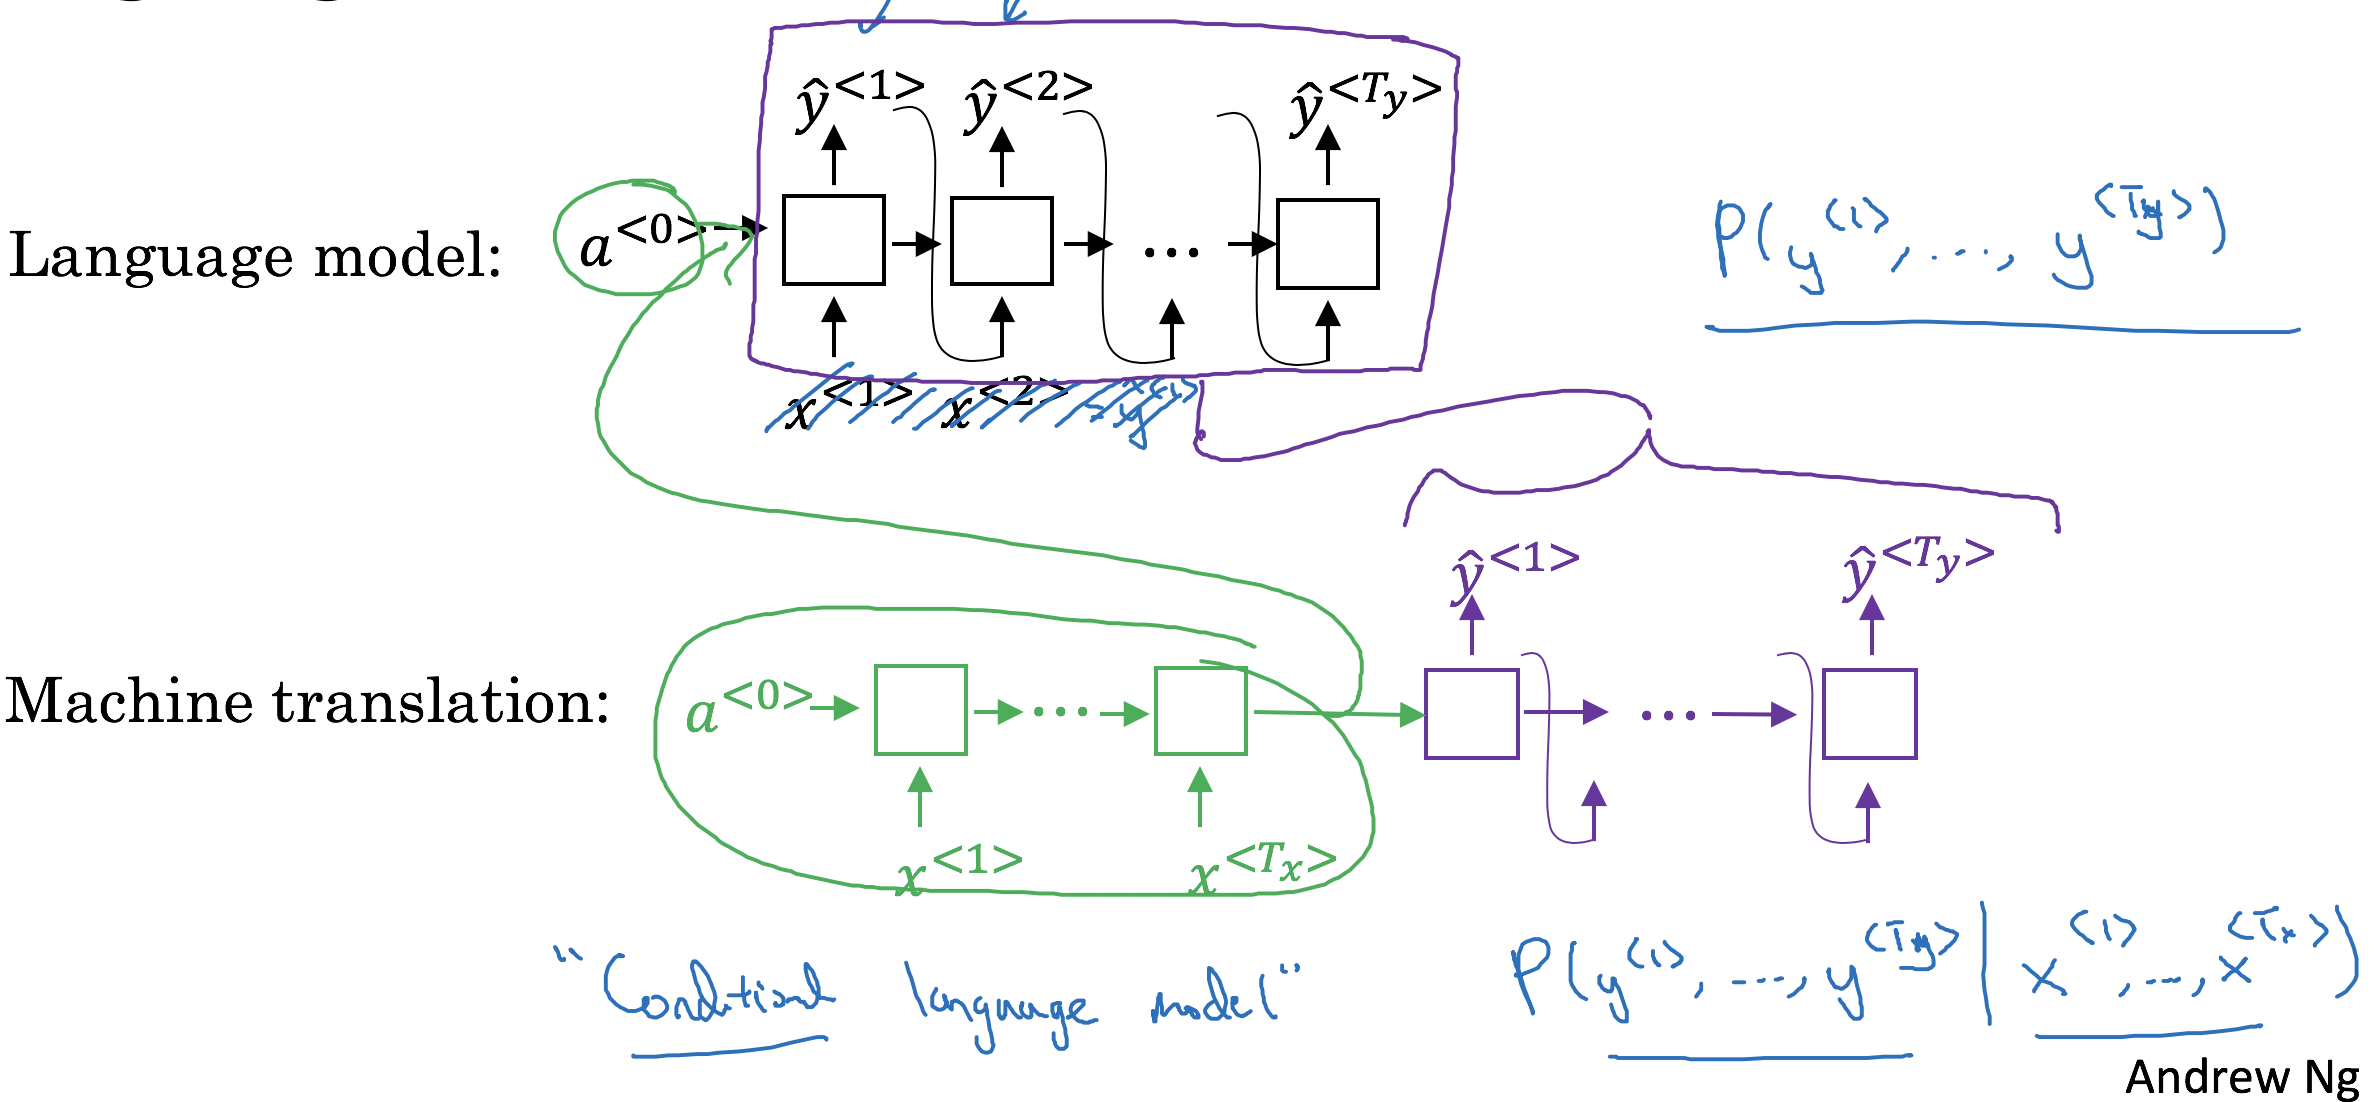
\includegraphics[scale=0.35]{Machine_Translation_Language_Model}
\caption{Machine translation can be thought as building a conditional language model}
\end{figure}
We don;t want to sample randomly, what you're looking for is a sentence that maximize

\begin{equation*}
\text{arg max }_{y^{1}, ..., y^{T_y}} P( y^{1}, ..., y^{T_y} | x)    
\end{equation*}
Why not a \textbf{Greedy Search} to solve this problem? i.e. pick a first word $P(\hat{y}^{<i>} | x)$, then pick second mosltly likely word, etc.

What do you want is to pick the entire sequence at once while maximizing the probability $P(\hat{y}^{<1>}, ..., \hat{y}^{<T_y>} | x)$ as it's not always optimal to pick a word at once. What you can use is an approximate search algorithm, as scanning the entire space.

\subsubsection{Beam Search}
Beam Search has a parameter B \texttt{beam width} (e.g. 3), it first selects the B most likely words and feed them into a segment of the encoding net, not really sure.

\begin{figure}[H]
\centering
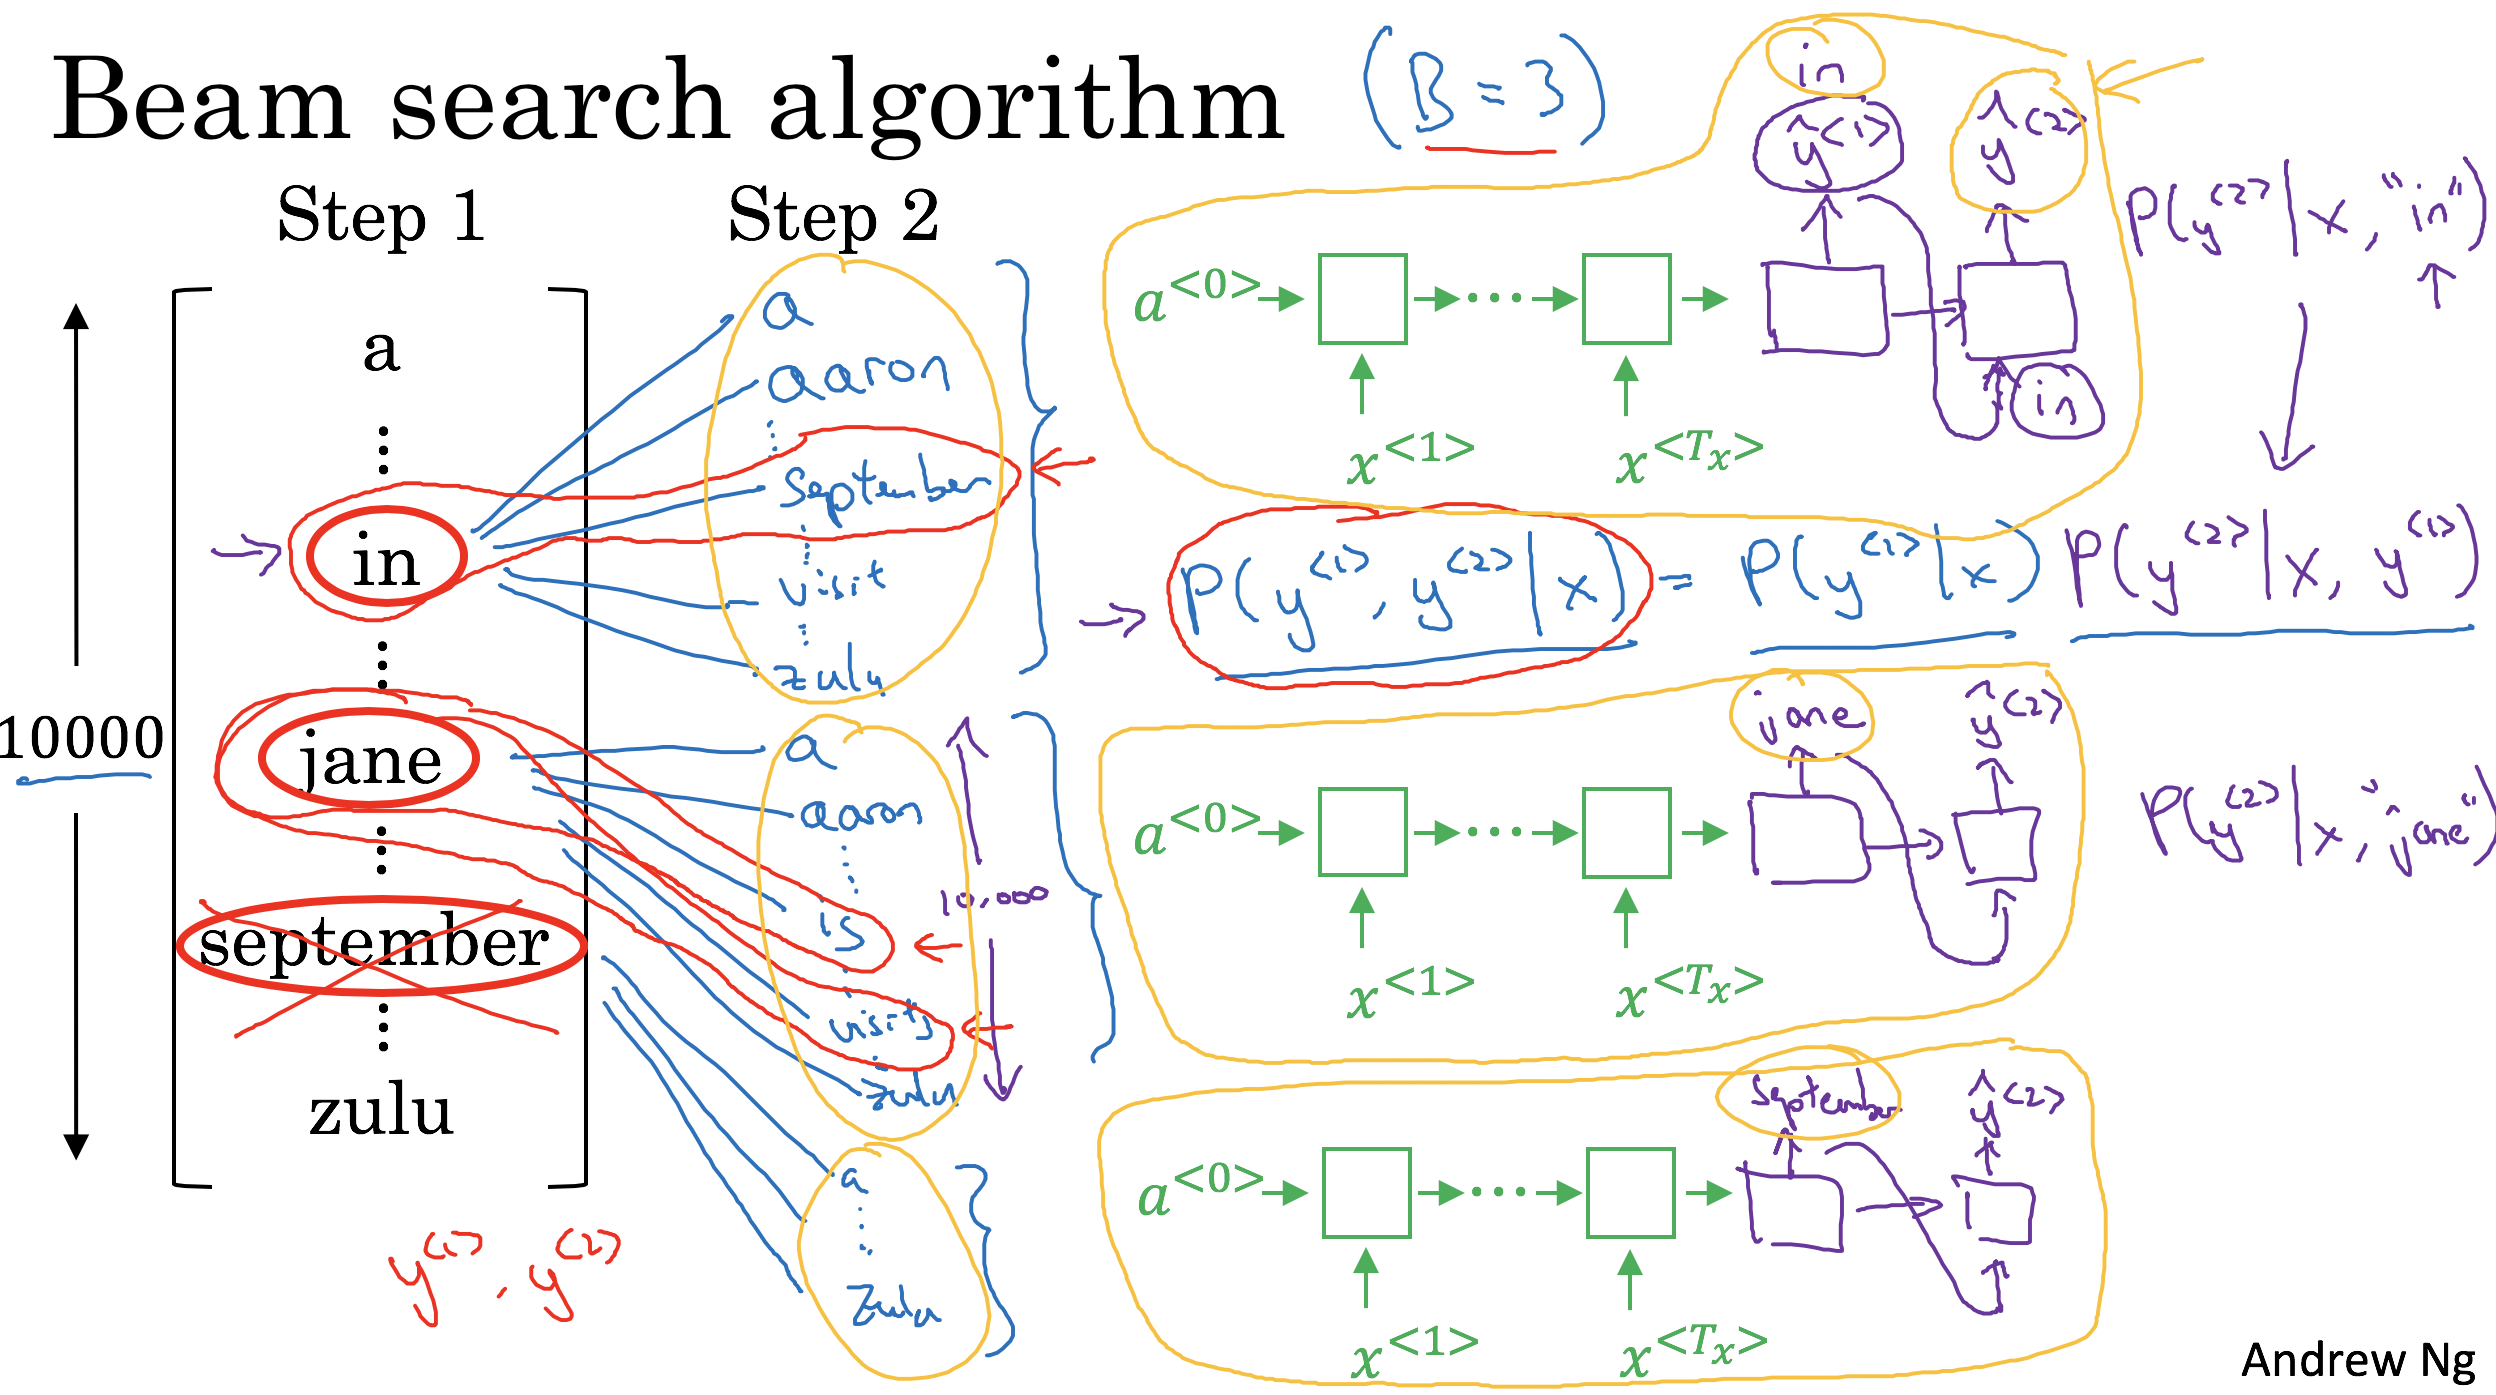
\includegraphics[scale=0.35]{Beam_Search}
\caption{Beam Search Algorithm}
\end{figure}
It will try to predict the probability of the third word to select, i.e. $\hat{y}^{<3>}$ given x (the french sentence to translate) and the english translation so far (e.g. 'in september'), i.e. $P(y^{<3>} | x, 'in september')$.

\subsubsection{Refinements to Beam Search}
Little changes to make Beam works better:
Length normalization

\begin{equation*}
\text{arg max}_{y} \Pi^{T_y}_{t=1} P(y^{<y>} | x, y^{<1>}, ..., y^{<t-1>})
\end{equation*}

All these number are too small, multiplying them return a really small number (that may underflow). In practice, we rather use the $\log$ function thus
\begin{equation*}
\text{arg max}_{y} \Pi^{T_y}_{t=1} \log P(y^{<y>} | x, y^{<1>}, ..., y^{<t-1>})
\end{equation*}
Another change to the above equation to futher optmize it, is to normalize by the legth of the sentence to avoid penalizing long sentences (where $\alpha$ is usually 0.7):
\begin{equation*}
\text{arg max}_{y} \frac{1}{T^{\alpha}_y} \Pi^{T_y}_{t=1} \log P(y^{<y>} | x, y^{<1>}, ..., y^{<t-1>})
\end{equation*}

\begin{itemize}
    \item If B is large, you tend to consider a lot of possibibilites and thus it's slower
    \item If B is small you endup with worst results but faster runtime
\end{itemize}
In production system, B is usually 10, at 100 it's too large for prod system. In research you can see up to 1000 as they aim to get the best performance.

\begin{quote}
    Unlike exact search algorithms like BFS (Breadth First Search) or  DFS (Depth First Search), Beam Search runs faster but is not guaranteed to find exact maximum for: arg $max_y P(y | x)$
\end{quote}

\subsubsection{Error analysis in beam search}
Error analysis on beam search

\begin{itemize}
    \item Human: Jane visits Africa in September. ($y^*$)
    \item Algorithm: Jane visited Africa last September. ($\hat{y}$)
\end{itemize}

\begin{itemize}
    \item Case 1: $P(y^* | x) > P(\hat{y} | x)$: Beam search chose $\hat{y}$. But $y^*$ attains higher $P(y | x)$. Conclusion: \textit{Beam search is at fault}.
    \item Case 2: $P(y^* | x) <= P(\hat{y} | x)$: $y^*$ is a better translation than $\hat{y}$. But RNN predicted $P(y^* | x) <= P(\hat{y} | x)$. Conclusion: \textit{RNN model is at fault}.
\end{itemize}
Figures out what faction of errors are "due to"" Beam Search vs. RNN model

\subsubsection{Bleu Score (optional)}
For a given french sentence, we may have multiple correct translations. One way to measure how good is this machine translation is by the Blue Score. Also called, Bilingual Evaluation understudy. A substitute for human evaluation

Clipping the count, is reducing the count of a unigram or bigram to the max count of it's appearance in one of Reference sentences.

\begin{equation}
P_1 = \frac{\sum_{unigram \in \hat{y}} Cout_{clip}(unigram)}{sum_{unigram \in \hat{y}} Cout(unigram)}
\end{equation}
n-grams
\begin{equation}
P_n = \frac{\sum_{n-gram \in \hat{y}} Cout_{clip}(n-gram)}{sum_{n-gram \in \hat{y}} Cout(n-gram)}
\end{equation}
\begin{quote}
     So the BP, or the brevity penalty, is an adjustment factor that penalizes translation systems that output translations that are too short.
\end{quote}

\subsubsection{Attention Model Intuition}
Till now we were using an architecture of encoding-decoding NN.


\begin{figure}[H]
\centering
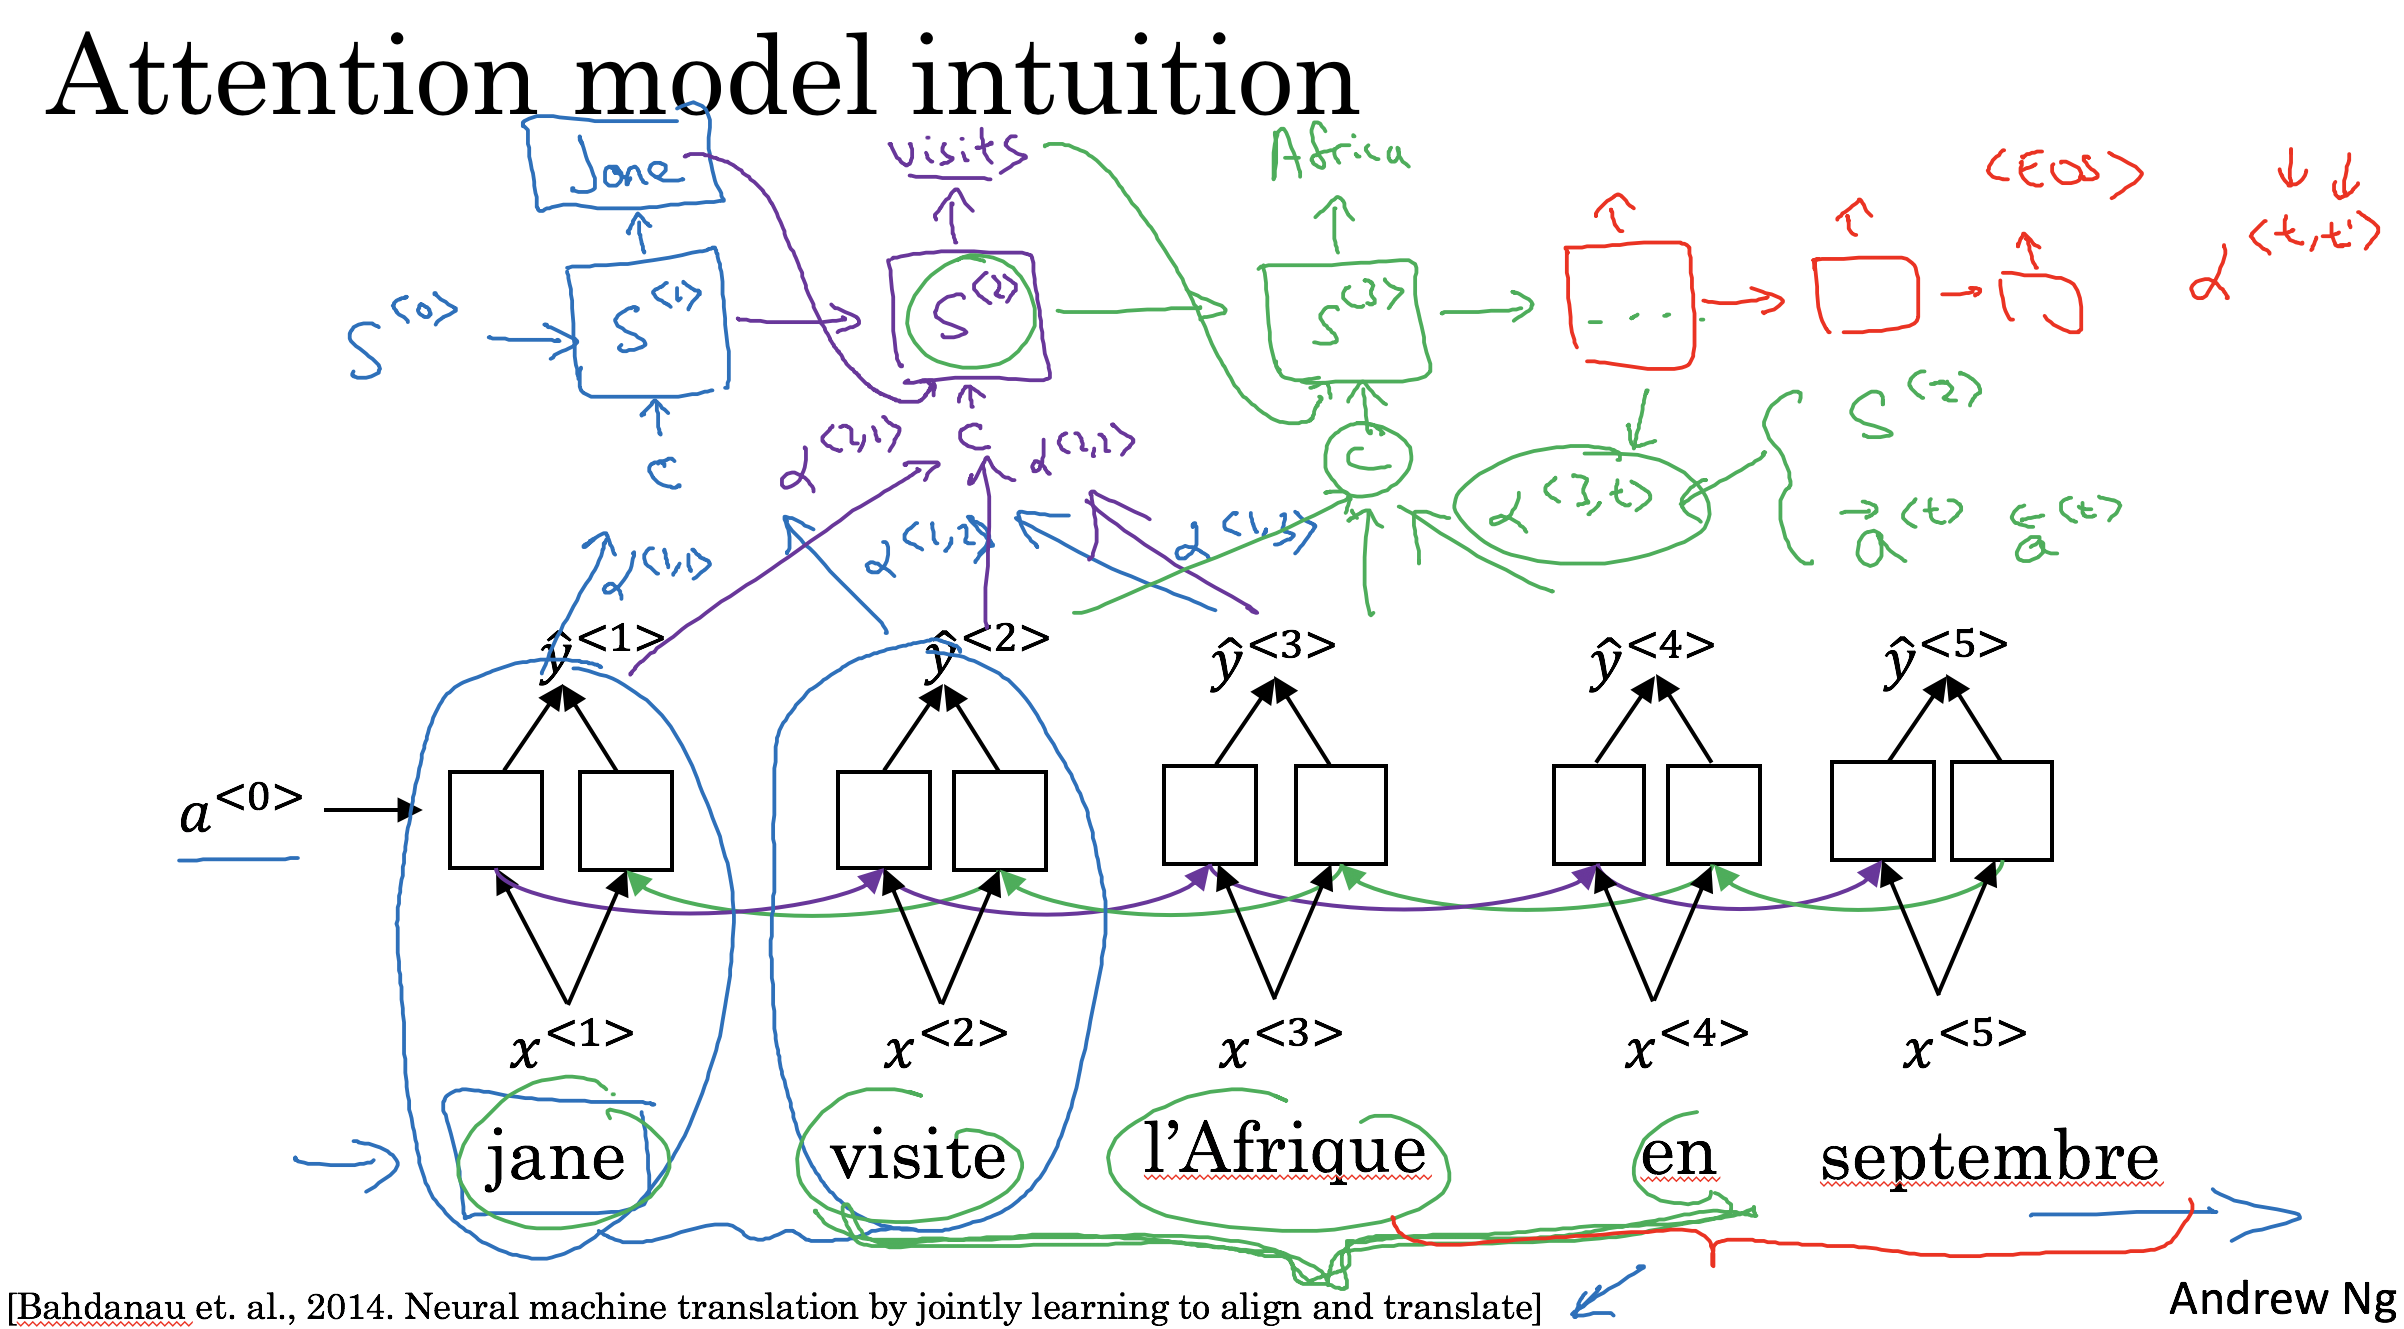
\includegraphics[scale=0.35]{Attention_Model_Intuition}
\caption{Attention model intuition}
\end{figure}

\subsubsection{Attention Model}
\begin{equation*}
    a^{<t'>} = (\overrightarrow{a}^{<t'>}, \overleftarrow{a}^{<t'>})
\end{equation*}
Computing attention $\alpha^{<t, t'>}$:

$\alpha^{<t, t'>}$ is amount of attention $y^<t>$ should pay to $a^{<t'>}$

\begin{equation*}
    \alpha^{<t, t'>} = \frac{\exp(e^{<t, t'>})}{\sum^{T_x}_{t'=1} \exp(e^{<t, t'>})}
\end{equation*}

This algorithms take quadric time to compute it's parameters.

\subsection{Speech recognition - Audio data}
\subsubsection{Speech recognition}
Attention algorithms.

CTC cost for speech recognition:
\begin{quote}
     if you have 10 seconds of audio and your features come at a 100 hertz so 100 samples per second, then a 10 second audio clip would end up with a thousand inputs. Right, so it's 100 hertz times 10 seconds, and so with a thousand inputs. But your output might not have a thousand alphabets, might not have a thousand characters.
\end{quote}
To address this issue, CTC inserts black words between characters.

\subsubsection{Trigger Word Detection}
\begin{figure}[H]
\centering
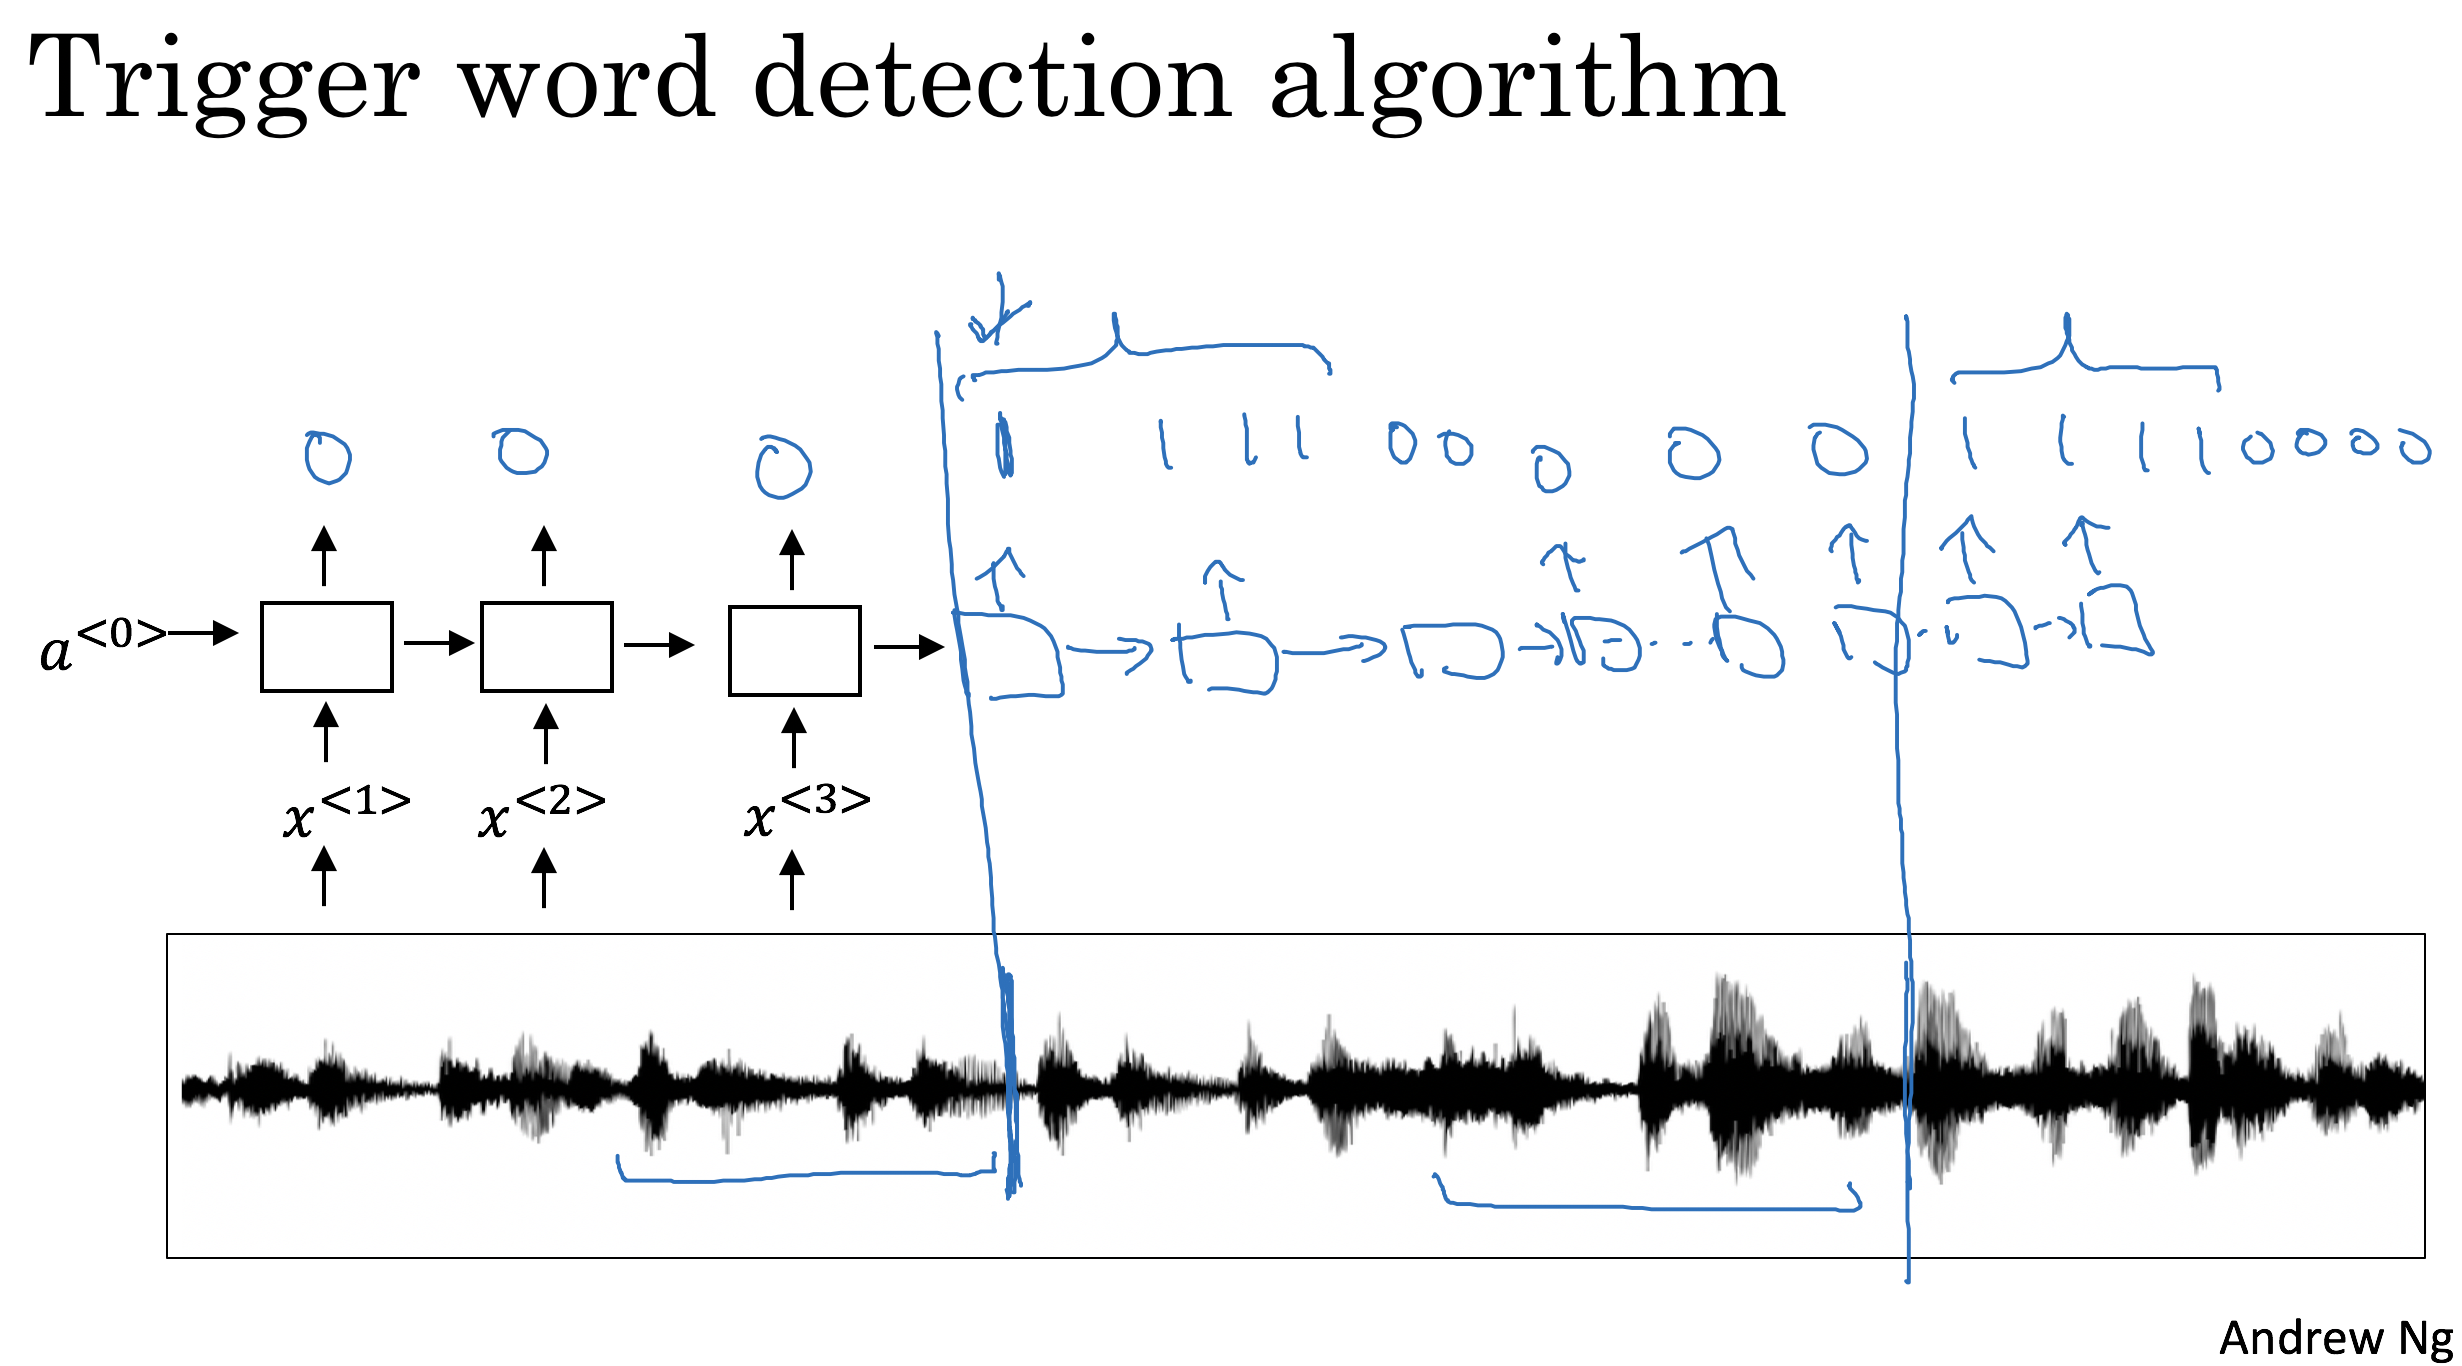
\includegraphics[scale=0.35]{Trigger_word_detection_algorithm}
\caption{Trigger word detection algorithm}
\end{figure}

\begin{quote}
     to wrap up in this course on sequence models you learned about rnns including both gr use and LS TMS and then in the second week you learned a lot about word embeddings and how they learn representations of words and then in this week you learned about the attention model as well as how to use it to process audio data
\end{quote}

\subsection{Conclusion}
Specialization outline
\begin{enumerate}
    \item Neural Networks and Deep Learning
    \item Improving Deep Neural Networks: Hyperparameter  
    tuning, Regularization and Optimization
    \item Structuring Machine Learning Projects
    \item Convolutional Neural Networks
    \item Sequence Models
\end{enumerate}

\subsection{Practice questions}
\subsubsection{QUIZ - Sequence models \& Attention mechanism}
\textbf{1.} Consider using this encoder-decoder model for machine translation.

This model is a “conditional language model” in the sense that the encoder portion (shown in green) is modeling the probability of the input sentence $x$.
\begin{itemize}
    \item True (X 1)
    \item False (X 2)
\end{itemize}
\textbf{2.} In beam search, if you increase the beam width BB, which of the following would you expect to be true? Check all that apply.
\begin{itemize}
    \item Beam search will run more slowly. (X)
    \item Beam search will use up more memory.
    \item Beam search will generally find better solutions (i.e. do a better job maximizing $P(y \mid x)$ (X 1)
    \item Beam search will converge after fewer steps.
\end{itemize}
\textbf{3.} In machine translation, if we carry out beam search without using sentence normalization, the algorithm will tend to output overly short translations.
\begin{itemize}
    \item True (X)
    \item False
\end{itemize}
\textbf{4.} Suppose you are building a speech recognition system, which uses an RNN model to map from audio clip xx to a text transcript $y$. Your algorithm uses beam search to try to find the value of $y$ that maximizes $P(y \mid x)$.

On a dev set example, given an input audio clip, your algorithm outputs the transcript $\hat{y}$ = "I'm building an A Eye system in Silly con Valley.", whereas a human gives a much superior transcript $y^*$ = "I'm building an AI system in Silicon Valley."

According to your model,


\begin{equation*}
P(\hat{y} \mid x) = 1.09*10^-7
\end{equation*}

\begin{equation*}
    P(y^* \mid x) = 7.21*10^-8    
\end{equation*}

Would you expect increasing the beam width B to help correct this example?
\begin{itemize}
    \item No, because $P(y^* \mid x) \leq P(\hat{y} \mid x)$ indicates the error should be attributed to the RNN rather than to the search algorithm. (X)
    \item No, because $P(y^* \mid x) \leq P(\hat{y} \mid x)$ indicates the error should be attributed to the search algorithm rather than to the RNN.
    \item Yes, because $P(y^* \mid x) \leq P(\hat{y} \mid x)$ indicates the error should be attributed to the RNN rather than to the search algorithm.
    \item Yes, because $P(y^* \mid x) \leq P(\hat{y} \mid x)$ indicates the error should be attributed to the search algorithm rather than to the RNN.
\end{itemize}
\textbf{5.} Continuing the example from Q4, suppose you work on your algorithm for a few more weeks, and now find that for the vast majority of examples on which your algorithm makes a mistake, $P(y^* \mid x) > P(\hat{y} \mid x)$. This suggest you should focus your attention on improving the search algorithm.
\begin{itemize}
    \item True. (X)
    \item False.
\end{itemize}
\textbf{6.} Consider the attention model for machine translation.
Further, here is the formula for $\alpha^{<t, t'>}$. Which of the following statements about $\alpha^{<t, t'>}$ are true? Check all that apply.
\begin{itemize}
    \item We expect $\alpha^{<t,t'>}$ to be generally larger for values of $a^{<t'>}$ that are highly relevant to the value the network should output for $y^{<t>}$. (Note the indices in the superscripts.) (X)
    \item We expect $\alpha^{<t, t'>}$ to be generally larger for values of $a^{<t>}$ that are highly relevant to the value the network should output for $y^{<t'>}$. (Note the indices in the superscripts.)
    \item $\sum_{t} \alpha^{<t, t'>} = 1$ (Note the summation is over $t$.)
    \item $\sum_{t'} \alpha^{<t, t'>} = 1$ (Note the summation is over t'.) (X)
\end{itemize}
\textbf{7.} The network learns where to “pay attention” by learning the values $e^{<t,t'>}$, which are computed using a small neural network: We can't replace $s^{<t-1>}$ with $s^{<t>}$ as an input to this neural network. This is because $s^{<t>}$ depends on $\alpha^{<t,t'>}$ which in turn depends on $e^{<t,t'>}$; so at the time we need to evalute this network, we haven’t computed $s^{<t>}$ yet.
\begin{itemize}
    \item True (X)
    \item False
\end{itemize}
\textbf{8.} Compared to the encoder-decoder model shown in Question 1 of this quiz (which does not use an attention mechanism), we expect the attention model to have the greatest advantage when:
\begin{itemize}
    \item The input sequence length $T_x$ is large. (X)
    \item The input sequence length $T_x$ is small.
\end{itemize}
\textbf{9.} Under the CTC model, identical repeated characters not separated by the "blank" character (\_) are collapsed. Under the CTC model, what does the following string collapse to?

\_\_c\_oo\_o\_kk\_\_\_b\_ooooo\_\_oo\_\_kkk
\begin{itemize}
    \item cokbok
    \item cookbook (X)
    \item cook book
    \item coookkboooooookkk
\end{itemize}
\textbf{10.} In trigger word detection, $x^{<t>}$ is:
\begin{itemize}
    \item Features of the audio (such as spectrogram features) at time $t$. (X)
    \item The $t$-th input word, represented as either a one-hot vector or a word embedding.
    \item Whether the trigger word is being said at time $t$.
    \item Whether someone has just finished saying the trigger word at time $t$.
\end{itemize}